\chapter{AreaComp}

\section{Konzept}

Sei $S = s_0, \dots, s_{n-1} \in \Sigma^*$ mit $n := |S|$ ein String über ein Alphabet $\Sigma$.

Ein Intervall $LCP[i..j]$ mit $0 \leq i \leq j < n$ im LCP-Array beschreibt wiederholte Vorkommen von Substrings. Aus diesem Intervall lässt sich schließen, wie oft dieser Substring vorkommt, wie lang dieser ist, und mithilfe des Suffix-Arrays lässt sich feststellen, wo dieser vorkommt. Jeder Eintrag $LCP[k], k \in 0$ im LCP-Array ist die Länge des längsten gemeinsamen Präfixes der beiden Suffixe ist, die bei $SA[k-1]$ und $SA[k]$ beginnen. Daher gilt dann folgendes:

An den Indizes $I = \{SA[i]\ |\ i \in \{i-1, \dots, j\}\}$ befindet sich jeweils ein Vorkommen eines Substrings der Länge $l = \min_{k = i, \dots, j} LCP[k]$. Wir nennen dann $W(i, j) := |I| = j - i + 2$ die Breite von $LCP[i..j]$ und $H(i, j) := l$ die Höhe von $LCP[i..j]$.\\\\
Intervalle mit großer Breite (viele Vorkommen) bzw. Höhe (langer Substring) bieten also eine besonders große Kompression, wenn diese Vorkommen durch ein Nichtterminal und eine entsprechende Produktionsregel ersetzt werden.

Es ist hier also eine Art Gütefunktion $A: \mathbb{N}_0 \times \mathbb{N}_0 \rightarrow \mathbb{N}_0$ nötig, die Intervalle je nach potentieller Kompression bewertet. Diese Funktion nennen wir Flächenfunktion. Je größer der von der Funktion gelieferte Wert, desto nützlicher ist das Intervall.\\\\
Die Idee ist also, inkrementell eine Straight Line Grammatik zu erzeugen. Dies geschieht durch die wiederholte Wahl eines vielversprechenden Intervall im LCP-Array anhand der Flächenfunktion. Jedes Vorkommen des von dem Intervall bestimmten Substring wird durch ein neues Nichtterminal und eine entsprechende neue Produktionsregel der Grammatik ersetzt.\\

Dies wird solange wiederholt bis keine Intervalle mehr übrig sind, die einen nützlichen Wert der Flächefunktion liefern. Etwa müssen Intervalle der Fläche $0$, bei der oben vorgeschlagenen Flächenfunktion nicht betrachtet werden.\\

Die Priorisierung von Intervallen anhand der Flächenfunktion kann mithilfe einer Prioritätswarteschlange umgesetzt werden. Die Intervalle werden mit dem Gewicht $A(i, j)$ eingefügt. So kann in jedem Durchlauf ein Element in der richtigen Reihenfolge entnommen werden.\\\\

\subsection{Beispiel}

Zunächst ein Beispiel für einen Durchlauf: Wir wählen die Flächenfunktion
\begin{equation}
	A[i, j] := \min \{ lcp[x]\ |\ i \leq x \leq j\} \cdot (j - i)
\end{equation} 
und betrachten den String $S =$ \enquote{ababcaba\$}. Dann gilt:

\begin{figure}[H]
	\centering
	\begin{tabular}{|c|c|c|l|} \hline
		$i$ & $SA$ & $LCP$ & Suffix\\ \hline
		$0$ & $8$ & $0$ & \$ \\\hline
		$1$ & $7$ & $0$ & a\$ \\\hline
		$2$ & $5$ & $1$ & aba\$ \\\hline
		$3$ & $0$ & $3$ & ababcaba\$ \\\hline
		$4$ & $2$ & $2$ & abcaba\$ \\\hline
		$5$ & $6$ & $0$ & ba\$ \\\hline
		$6$ & $1$ & $2$ & babcaba\$ \\\hline
		$7$ & $3$ & $1$ & bcaba\$ \\\hline
		$7$ & $4$ & $0$ & caba\$ \\\hline
	\end{tabular}
\end{figure}

Wir beginnen mit der leeren Grammatik $S \rightarrow ababcaba\$$. Die Intervalle mit maximalem $A$ sind $LCP[2..3]$ und $LCP[3..3]$. $A(2, 3) = A(3, 3) = 6$.\\
Wählt man nun das Intervall $LCP[3..4]$ so gilt entsprechend $W(3, 4) = 3$ und $H(3, 4) = 2$. Der zu ersetzende Substring ($ab$) ist also zwei Zeichen lang und kommt dreimal im String vor.\\
Wir erzeugen nun eine neue Produktionsregel $A \rightarrow ab$ und ersetzen jedes Vorkommen von $ab$ in der Grammatik durch $A$.
Die resultierende Grammatik ist dann also:
\begin{align*}
	S &\rightarrow AAcAa\\
	A &\rightarrow ab
\end{align*}

Es gibt nun keine wiederholten Zeichenfolgen mehr und der Algorithmus terminiert.

\subsection{Überlegungen}

\subsubsection{Überlappungen}

Es kann vorkommen, dass ein zu ersetzendes Muster überlappend vorkommt, wie etwa $aa$ im String $aaa$. In diesem Fall können die überlappenden Vorkommen nicht ersetzt werden. Hier muss also Acht gegeben werden. Gegebenfalls müssen also alle Positionen ignoriert werden, die sich überlappen.

\subsubsection{Überschneidende Substitutionen}

Es können aber auch in einem Schritt eine Substitution durch ein LCP-Intervall $I_1 := LCP[i_1..j_1]$ durchgeführt worden sein, die sich mit einer späteren Substitution durch ein LCP-Intervall $I_2 := LCP[i_2..j_2]$ überschneiden. In diesem Fall, kann der tatsächliche Nutzen der Substitution sinken. Es muss also dafür gesorgt werden, dass bereits ersetzte Teile des Strings nicht nochmals ersetzt werden.


\section{AreaComp V1}

Die erste Version ist eine naive Implementierung. Der Algorithmus verwaltet eine Menge von Regeln. In jedem Durchlauf wird nacheinander jede Regel $(X \rightarrow w) \in P$ aus der Menge entnommen und das Suffix- und LCP-Array für die rechte Seite dieser Regel berechnet. Es wird nun eine Prioritätswarteschlange erzeugt, die alle möglichen LCP-Intervalle enthält. Das beste LCP-Intervall wird daraus entnommen. Sei $p \in (N \cup \Sigma)^*$ das, durch das LCP-Intervall bestimmte, zu ersetzende Muster. Die Indizes, an denen ein Vorkommen von $p$ in $w$ existiert, kann einfach mithilfe des Suffix- und LCP-Array berechnet werden.

Es werden nun alle bestimmten Vorkommen darauf untersucht, ob sich diese mit Anderen überschneiden. Hierzu werden die Indizes, an denen $p$ vorkommt, aufsteigend sortiert und durchlaufen. Dabei werden alle Indizes gelöscht, die einen Abstand von weniger als $|p|$ zum letzten Index haben, gelöscht. Damit bleiben nur Vorkommen übrig, die sich nicht überschneiden. Sind nun nur noch weniger als zwei Positionen übrig, so wird das nächst-beste LCP-Intervall aus der Warteschlange entnommen und der Vorgang wiederholt. Sind keine Intervalle mehr übrig, so fahre zur nächsten Produktionsregel fort.

Der von diesem Intervall bestimmte Substring wird dann durch ein neues Nichtterminal und eine zugehörige Produktionsregel ersetzt. Zu diesem Zweck wird die gesamte Grammatik nach Vorkommen durchsucht und diese durch das Nichtterminal ersetzt.

Die Datenstruktur, mit der Regeln, Terminale und Nichtterminale verwaltet werden, ist gleich der Datenstruktur, die Sequitur benutzt. Allerdings verwendet der Algorithmus zusätzlich eine Hashtabelle, die eine ID auf ihre zugehörige Regel abbildet.

Diese Implementierung hat nicht das Problem, dass sich überschneidende Substitutionen entstehen können, da Suffix- und LCP-Array für jede Regel symbolweise neu erzeugt werden. 

\subsection{Probleme}

\subsubsection{Laufzeit}
Das größte Problem dieser Implementierung ist die Laufzeit. Sei $s \in \Sigma^*$ mit $n := |s|$ $\mathcal{O}(n)$ der Eingabestring.

In jedem Durchlauf wird für jede Regel $X \rightarrow w \in P, X \in N, w \in (N \cup \Sigma)^*$ das im Bezug auf die Flächenfunktion beste LCP-Intervall berechnet. Dessen Berechnung dominiert die Laufzeit dieser Version des Algorithmus. 
Es existieren $|w|^2$ solche Intervalle.
Für jedes dieser Intervalle muss die Flächenfunktion berechnet werden. Eine Flächenfunktion, die alle Werte in ihrem gegebenen Intervall $I$ in Betracht zieht, muss mindestens eine Laufzeit von $\mathcal{O}(|I|)$ haben. Betrachten wir die Länge aller möglichen LCP-Intervalle, so ist deren Gesamtlänge $\mathcal{O}(|w|^3)$. Folglich ist die Gesamtlaufzeit der Flächenfunktionsaufrufe pro Produktionsregel und Durchlauf $\mathcal{O}(|w|^3)$. 

Da die Gesamtlänge der Grammatik $n$ nicht überschreiten kann, ist die Laufzeit der Flächenfunktionsaufrufe pro Durchlauf $\mathcal{O}(n^3)$. 

In jedem Durchlauf, in dem eine Substitution möglich ist, wird mindestens eine Substitution durchgeführt. Da durch jede Substitution die Grammatik um mindestens $1$ Zeichen kleiner wird (entweder mindestens $2$ Vorkommen der Länge mindestens $3$ oder mindestens $2$ Vorkommen der Länge mindestens $2$), können im Worst-Case insgesamt $\mathcal{O}(n)$ Durchläufe stattfinden.

Insgesamt resultiert also eine sehr hohe Laufzeit von etwa $\mathcal{O}(n^4)$.

\subsubsection{Erkennung von Wiederholungen}

Diese Version des Algorithmus erkennt keine wiederholten Vorkommen von Substrings, falls diese in verschiedenen Produktionsregeln auftreten.
Etwa würde in der folgenden Grammatik das wiederholte Vorkommen von $abc$ nicht erkannt werden:

\begin{align*}
	S &\rightarrow AA\textcolor{red}{abc}\\
	A &\rightarrow cdef\textcolor{red}{abc}
\end{align*}

Dies liegt daran, dass das Suffix- und LCP-Array, in dem nach wiederholten Vorkommen gesucht wird, für jede Produktionsregel einzeln berechnet werden. Dabei werden natürlich alle Vorkommen außerhalb dieser Produktionsregel nicht erfasst.

\section{AreaComp V2}


Gegenüber der ersten Version des Algorithmus gibt es mehrere Verbesserungen:

\subsection{Datenstrukturen} Regeln bestehen nun nicht mehr aus der verketteten Struktur wie bei Sequitur. Stattdessen besitzt eine Produktionsregel nun zwei dynamische Arrays. \texttt{symbols} enthält die Symbole und \texttt{cumulativeLength} ist die Präfixsumme über die (voll expandierte) Länge der einzelnen Symbole in der Symbolliste.

Sei zum Beispiel die Grammatik: 
\begin{align*}
	A &\rightarrow BBde\\
	B &\rightarrow abc
\end{align*}
Dann gilt für die Produktionsregel $A$: 
\begin{align*}
	\texttt{symbols} &= [B, B, d, e]\\
	\texttt{cumulativeLength} &= [3, 6, 7, 8]
\end{align*}

\subsection{Suffix- und LCP-Array}
Im Gegensatz zu Version 1 wird in Version 2 das Suffix- und LCP-Array, und damit auch die Prioritätswarteschlange, nur einmal zu Anfang des Algorithmus global für den Eingabestring berechnet. Damit wird die wiederholte Berechnung in jedem Durchlauf gespart. 
Dadurch wird ebenfalls das Problem behoben, dass V1 wiederholte Vorkommen, die nicht in derselben Regel liegen, nicht erfasst.

Dies hat allerdings auch Auswirkungen auf den Algorithmus, die neue Probleme schaffen. Im Gegensatz zu den in V1 berechneten Suffix- und LCP-Arrays, ändern sich das Suffix- und LCP-Array in V2 nicht, wenn Substitutionen stattfinden. 

Sei $s = s_0, \dots, s_{n-1} \in \Sigma^*$ mit $n := |s|$ der Eingabestring und $p \in \Sigma^*$ mit $l := |p|$  ein zu substituierendes Muster und $id_p \in \mathbb{N}$ die ID der Regel, die auf $p$ abbildet. Zusätzlich sei $i \in \mathbb{N}, 0 \leq i \leq n - l$ ein Index in $s$. Wird nun ein Vorkommen von $p$ in $s$ bei Index $i$ ersetzt, so heißt das Intervall $R_{ID_p, i} := [i, i + l - 1]$ Ersetzungsintervall der Regel $id_p$ bei Index $i$. Dabei wird $R_{0, 0} = [0, n-1]$ zu Beginn des Algorithmus erzeugt, wobei $R_0$ die Startregel ist. \\

\subsection{Neue Datenstrukturen}
Wir führen nun zwei Datenstrukturen ein: 
\begin{itemize}[leftmargin=10em]
	\item[\texttt{ruleIntervals}] ist eine Liste, die für jeden Index $i \in \{0, \dots, n - 1\}$ eine Liste der IDs derjeniger Regeln, für die ein Ersetzungsintervall existiert, das diesen Index einschließt. Dabei sind die IDs in der Reihenfolge der Verschachtelung der Ersetzungsintervalle. Je tiefer verschachtelt das Ersetzungsintervall ist, desto höher der Index in der Liste.\\ 
	Anders formuliert, beinhaltet die Liste die Indizes aller Regeln, die von der Startregel ausgehend in der Grammatik durchlaufen werden müssen, um das Zeichen an Index $i$ im Eingabestring zu erreichen, genau in der Reihenfolge in der sie durchalufen wurden. Es ist also der letzte Index immer die Regel-ID, der dem am tiefsten verschachtelten Ersetzungsintervall zugehörigen Regel. 
	
	Sei die Grammatik beispielhaft: (Startregel $R0$)
	\begin{align*}
		R_0 &\rightarrow R_2\ c\ R_2\\
		R_1 &\rightarrow a\ a\\
		R_2 &\rightarrow R_1\ b\ R_1
	\end{align*}
	Dann ist der vollständig expandierte String $aabaacaabaa$. Der Eintrag in \texttt{ruleIntervals} für den Index $1$ ist dann also $[0, 2, 1]$, da wir die Regeln in der Reihenfolge $R_0 \rightarrow R_2 \rightarrow R_1$ durchlaufen müssen, um das $a$ an Index $1$ zu erreichen.
	
	\item[\texttt{ruleIntervalStarts}] ist eine Hashtabelle, die von einem Index $i \in \{0, \dots, n - 1\}$ auf eine Menge von Regel-IDs abbildet. Dabei befindet sich eine Regel-ID genau dann in \texttt{ruleIntervalStarts}$[i]$, wenn es ein Ersetzungsintervall für diese Regel-ID gibt, das an diesem Index beginnt.
	
	Diese Datenstruktur dient dem Zweck, bestimmen zu können an welchem Index ein Ersetzungsintervall beginnt. Falls zwei Ersetzungsintervalle der gleichen Regel ohne Lücke aufeinanderfolgen, dann kann aus \texttt{ruleIntervals} allein nicht mehr bestimmt werden, an welchem Index dieses Intervall nun beginnt. In diesem Fall sind diese zwei aufeinander folgenden Intervalle nicht von einem großen Intervall zu unterscheiden.
\end{itemize}

\subsection{Substitution}
Wird nun $p$ in $s$ am Index $i$ substituiert, so wird nun $id_p$ in \texttt{ruleIntervals} in die Listen der Indizes $i$ bis $i + l - 1$ an die richtige Stelle eingefügt, sowie auch in \texttt{ruleIntervalStarts}$[i]$.

Nachdem alle Positionen festgestellt wurden, an denen das Muster $p$ vorkommt, werden, wie bei V1, sich überschneidende Vorkommen entfernt. Daraufhin wird geprüft, ob die Substitution an den übrigen Indizes möglich ist. Dies wird mithilfe von \texttt{ruleIntervals} und \texttt{ruleIntervalStarts} bewältigt.

\subsubsection{Bedingungen für Substitution} Eine Substitution von $p$ an Index $i$ ist genau dann möglich, wenn folgende Bedingungen gelten:

\begin{enumerate}
	\item Die IDs der tiefsten verschachtelten Regeln bei jeweils den Indizes $i$ und $i + l - 1$ müssen übereinstimmen.
	\item Die Startindizes der Ersetzungsintervalle der tiefsten verschachtelten Regeln bei jeweils den Indizes $i$ und $i + l - 1$ müssen übereinstimmen. 
\end{enumerate}

Diese Bedingungen zusammen garantieren, dass das Vorkommen von $p$ in demselben Ersetzungsintervall beginnt, in dem es auch endet. Nur in diesem Fall darf dieses Vorkommen substituiert werden. Ansonsten, müssten Teile unterschiedlicher Produktionsregeln durch \textit{ein} Nichtterminal ersetzt werden. Dies ist nicht möglich.\\\\
Ob ein Vorkommen diese Bedingungen erfüllt, wird folgendermaßen geprüft:

Die IDs der tiefsten verschachtelten Regeln lassen sich leicht mit einem Look-Up in \texttt{ruleIntervals} an den Indizes $i$ und $i + l - 1$ bestimmen. Die IDs sind dann jeweils die letzten Elemente in den abgerufenen Listen.

Die Startindizes der Ersetzungsintervalle werden bestimmt, indem für die beiden Indizes jeweils die ID $id_T \in \mathbb{N}$ der tiefsten Regel an diesem Index bestimmt wird. Von diesem Index wird solange zurückgelaufen, bis ein Eintrag in \texttt{ruleIntervalStarts} existiert, der $id_T$ enthält.

\subsubsection{Unterschiedliche Vorkommen}

Es existiert aber nun ein weiteres Problem. Betrachten wir beispielsweise die Grammatik für den String $abcabcde$:

\begin{align*}
	R_0 &\rightarrow R_1\ R_1\ d\ e\\
	R_1 &\rightarrow a\ b\ c
\end{align*}

Da das Suffix- und LCP-Array global sind, könnte der Algorithmus als nächstes die beiden Vorkommen von $ab$ finden. 
Allerdings fällt hier auf, dass diese Vorkommen schon durch die Substitution von $R1$ auf ein einziges Vorkommen innerhalb der Grammatik reduziert wurde. Demnach, darf $ab$ nicht nochmals ersetzt werden. 
Es muss nun möglich sein zu überprüfen, ob es Vorkommen gibt, die tatsächlich auch \textit{in der Grammatik} mehrmals vorkommen.
Dies kann mit dem folgenden Algorithmus festgestellt werden:

\begin{algorithm}
	\caption{differingOccurrences}
	\begin{algorithmic}
		\REQUIRE $positions:$ Liste von Startindizes
		\STATE $firstRuleId \leftarrow -1$
		\STATE $set \leftarrow \emptyset$
		\FOR {$i$ \textbf{in} $positions$}
			\STATE $ruleId \leftarrow \text{Regel-ID des Ersetzungsintervall bei } i$
			\STATE $startIndex \leftarrow \text{Startindex des Ersetzungsintervall bei } i$
			
			\IF {$firstRuleId = -1$}
				\STATE $firstRuleId \leftarrow ruleId$
			\ELSIF {$ruleId \neq firstRuleId$ \OR $startIndex \in set$}
				\RETURN \TRUE
			\ENDIF
			\STATE $set \leftarrow set \cup \{startIndex\}$
		\ENDFOR
		\RETURN \FALSE
	\end{algorithmic}
\end{algorithm}

Wir speichern die erste Regel-ID, der wir begegnen. Kommt später eine andere Regel-ID vor, so müssen die Vorkommen von $p$ zwangsweise unterschiedlich sein und der Algorithmus gibt $\texttt{true}$ zurück.
Wir iterieren durch die Indizes, an denen $p$ vorkommt.Für jeden dieser Indizes $j \in \mathbb{N}$ bestimmen wir den Anfangsindex des tiefsten Ersetzungsintervalls bei $j$. 
Falls wir diesen Anfangsindex noch nicht gesehen haben, speichern wir diesen. Falls doch, brechen wir ab und geben $\texttt{true}$. 
Dies ist korrekt, denn angenommen, wir befinden uns bei Index $j$ und der Anfangsindex des Ersetzungsintervalls ist $i < j$. Es gelte auch, dass wir $i$ als bereits gespeichert vorfinden. Dann gibt es also einen Index $k$ mit $i \leq k < j$, so dass $k$ und $j$ in Ersetzungsintervallen liegen, die denselben Anfangsindex besitzen. Dann sind zwei Fälle möglich:

\begin{enumerate}
	\item[\textbf{Fall 1}] Die Regel-IDs der beiden Intervalle sind gleich.\\
	In diesem Fall sind die Intervalle gleich. Da $k < j$ gilt, gibt es also in derselben Regel mindestens zwei Vorkommen von dem Muster $p$. Damit kann der Algorithmus also terminieren und $\texttt{true}$ zurückgeben.
	\item[\textbf{Fall 2}] Die Regel-IDs sind unterschiedlich.\\
	Dieser Fall wird durch die Bedingung $ruleId \neq firstRuleId$ bemerkt und der Algorithmus gibt korrekterweise $\texttt{true}$ zurück.
\end{enumerate}

Falls kein Startindex eines Intervalls doppelt gefunden wird und alle gefundenen Ersetzungsintervalle dieselbe Regel-ID besitzen, gibt der Algorithmus $\texttt{false}$ zurück.

\subsubsection{Faktorisieren}

Nach der Vorbearbeitung durch die beschriebenen Vorgänge müssen jetzt nur noch eine neue Produktionsregel erstellt werden, die $p$ Produziert, und die Vorkommen durch das zugehörige Nichtterminal ersetzt werden.

Hierzu wird ein Index $i$, an dem $p$ vorkommt, aus dem Array entnommen. Es ist wichtig zu beachten, dass diese Indizes Positionen im Eingabetext beschreiben. Es muss dieser Index also so vorverarbeitet werden, um den tatsächlichen lokalen Index des Startsymbols in der Regel zu erhalten, in der das Vorkommen ersetzt werden muss.

Um dies zu lösen, kommt eine binäre Suche auf der \texttt{cumulativeLength} Liste zum Einsatz. Da dort die Präfixsumme über die Längen der einzelnen Symbole in \texttt{symbols} gespeichert ist, 
lässt sich also derjenige lokale Index $j$ in der Regel bestimmen, so dass in der voll expandierten Form des Symbols $\texttt{symbols}[j]$ das Terminal $s_{i}$ zu finden ist.
Von dort an kann dann durch Iterieren durch $\texttt{symbols}$ die erforderliche Anzahl an Symbolen durch das neue Nichtterminal ersetzt werden.
Ebenfalls wird dann in $\texttt{ruleIntervals}$ und $\texttt{ruleIntervalStarts}$ der Bereich markiert, der nun von der Regel ersetzt wurde, in dem die ID der neuen Regel an die entsprechenden Stellen eingefügt wird.

\subsection{Probleme}

\subsubsection{Laufzeit}

Wie bei V1 ist auch bei V2 die Laufzeit noch unzureichend. Zwar entfallen durch die neuen Datenstrukturen etwa das wiederholte Neuberechnen des Suffix- und LCP-Arrays und die Scans durch die gesamte Grammatik.

Allerdings zieht V2 immer noch die $\mathcal{O}(n^2)$ vielen Teilintervalle des LCP-Arrays in betracht. Von diesen Intervallen sind bei weitem nicht alle von Nutzen. Dadurch ergibt sich immer noch eine sehr schlechte Laufzeit.

\section{AreaComp V3}

In Version 3 des Algorithmus werden die Wahl der LCP-Intervalle, die in Betracht gezogen werden sollen, eingeschränkt. Ebenfalls wird effizienteres Markieren von Ersetzungsintervallen mithilfe einer neuen Datenstruktur, basierend auf einer Predecessor-Datenstruktur, möglich gemacht. 

\subsection{Wahl der LCP-Intervalle}

Die Grundlage hierfür bieten die Maximalen LCP-Intervalle von Abouelhoda et al. \cite{abouelhoda_optimal_2002}.\\
Sei beispielsweise folgendes Array, das LCP-Array eines Eingabetextes. 
\begin{figure}[H]
	\centering
	\begin{tikzpicture}
		
		\matrix (A) [matrix of nodes, nodes={draw, minimum size=5mm, anchor=center}, nodes in empty cells, column sep=-\pgflinewidth, right=1cm of Symbols]{
			0 & 1 & 2 & 2 & 3 & 0 & 1 & 0\\
		};
	\end{tikzpicture}
\end{figure}
Es gilt nun zu entscheiden, welche Intervalle im zugehörigen Suffix-Array einen wiederholt auftretenden Substring bezeichen, dessen Substitution eine möglichst gute Kompression erzielt.

Etwa wäre das Intervall $[1..3]$ keine sinnvolle Wahl. Das längste gemeinsame Präfix auf diesem Intervall ist $2$, da $LCP[2] = 2$ und $LCP[3] = 2$. Allerdings kann das Intervall auch $[1..4]$ gewählt werden, ohne die Länge des längsten gemeinsamen Präfix zu verringern, da auch $LCP[4] \geq 2$ ist. 
Es folgt also, dass es keinen Nutzen hat, das Intervall $[1..3]$ gegenüber $[1..4]$ zu betrachten.

Wir benötigen also nur die lokal größtmöglichen Intervalle, die für einen bestimmten längsten gemeinsamen Präfix möglich sind. Die maximalen LCP-Intervalle aus \cite{abouelhoda_optimal_2002} dienen diesem Zweck. Durch das Kind-Array können all diese LCP-Arrays bestimmt werden, indem für jedes maximale LCP-Intervall die Kind-Intervalle bestimmen werden, und dies rekursiv fortgesetzt wird.

Für unsere Zwecke sind natürlich nur $l-$Intervalle von Bedeutung, für die $l \geq 2$ gilt, da Substrings mit Länge kleiner als zwei keine mögliche Kompression durch Substitution bieten.

Es werden also nun statt allen möglichen Intervallen, nur die maximalen LCP-Intervalle berechnet, indem rekursiv die Kind-Intervalle des Wurzel-Intervalls ($[0..n]$) berechnet werden. Damit reduziert sich die Anzahl der Intervalle auf $\mathcal{O}(n)$.

\subsection{RuleIntervalIndex}

Ein weiteres Problem sind die Datenstrukturen $\texttt{ruleIntervals}$ und $\texttt{ruleIntervalStarts}$. Diese sind sowohl im Bezug auf Speicher als auch Laufzeit ineffizient. Die Lösung für dieses Problem bietet die Datenstruktur $\texttt{RuleIntervalIndex}$.

Diese basiert auf einer assoziativen Predecessor-Datenstruktur \cite{dinklage_engineering_2021} und unterstützt auch entsprechende Anfragen. Hier wird zu diesem Zweck eine assoziative Variante von Red-Black-Trees \cite{bayer_symmetric_1972, guibas_dichromatic_1978} verwendet (\texttt{TreeMap} in Java). Diese hat eine Laufzeit von $\mathcal{O}(\log n)$ bei allen Operationen der Predecessor-Datenstruktur. Die Elemente der Datenstruktur sind Teile von Ersetzungsintervallen und die Schlüssel die Startindizes der Intervall-Teile. Diese enthalten folgende Attribute:
\begin{itemize}[leftmargin=2.5cm]
	\item[\texttt{ruleId}] Die ID der Regel, die dieses Intervall repräsentiert
	\item[\texttt{start}] Der Start-Index dieses Intervall-Teils
	\item[\texttt{end}] Der End-Index dieses Intervall-Teils
	\item[\texttt{totalStart}] Der Start-Index des gesamten Ersetzungsintervall, dem dieser Teil angehört
\end{itemize}


Es wird immer jeweils das am tiefsten verschachtelte Intervall pro Bereich in der darunterliegenden Predecessor-Datenstruktur gespeichert gespeichert. Betrachte beispielhaft die folgende Grammatik für den String $abcdbcabcde$:

\begin{align*}
	R_0 &\rightarrow R_1 R_2 R_1 e\\
	R_1 &\rightarrow a R_2 d\\
	R_2 &\rightarrow bc
\end{align*}

Die Datenstrukturen aus V2 wären dann:

\begin{figure}[H]
	\centering
	
	\subfloat[][\texttt{ruleIntervals}]{
		\scalebox{.9}{
			\begin{tabular}{|c|c|c|c|c|c|c|c|c|c|c|} \hline
				$0$ & $0$ & $0$ & $0$ & $0$ & $0$ & $0$ & $0$ & $0$ & $0$ & $0$ \\\hline
				$1$ & $1$ & $1$ & $1$ & $2$ & $2$ & $1$ & $1$ & $1$ & $1$ & \\\hline
				& $2$ & $2$ &     &     &     &     & $2$ & $2$ &     & \\\hline
			\end{tabular} 
		}
 	}
	\quad
 	\subfloat[][\texttt{ruleIntervalStarts}]{
 		\scalebox{.9}{
	 		\begin{tabular}{|c|c|c|c|c|c|c|c|c|c|c|} \hline
	 			$\{0, 1\}$ & $\{2\}$ & & & $\{2\}$ & & $\{1\}$ & $\{2\}$ & & & \\\hline
	 		\end{tabular} 
 		}
 	}
\end{figure}

Dagegen sieht $\texttt{RuleIntervalIndex}$ folgendermaßen aus (die Baumstruktur wird hier aus Gründen der Leserlichkeit ausgelassen):

\begin{figure}[H]
	\centering
	
	\begin{tikzpicture}
		
		\matrix (A) [matrix of nodes, nodes={draw, minimum size=7mm, anchor=center}, column sep=-\pgflinewidth]{
			$R_1$-$[0..0]$ & $R_2$-$[1..2]$ & $R_1$-$[3..3]$ & $R_2$-$[4..5]$ & $R_1$-$[6..6]$ & $R_2$-$[7..8]$ & $R_1$-$[9..9]$ & $R_0$-$[10..10]$\\
		};
		
	\end{tikzpicture}
\end{figure}

So kann der Speicherverbrauch gegenüber $\texttt{ruleIntervals}$ und $\texttt{ruleIntervalStarts}$ verringert werden. Allerdings verbessert sich auch die Laufzeit.

\subsubsection{Operationen}

$\texttt{RuleIntervalIndex}$ unterstützt die folgenden Operationen:

\begin{itemize}[leftmargin=5cm]
	\item[$\texttt{mark(id, start, end)}$] Fügt ein neues Ersetzungsintervall $[start.. end]$ in die Datenstruktur ein für die Regel-ID $\texttt{ruleid}$. Dies ist die aufwendigste Operation dieser Datenstruktur. Einerseits können die Grenzen $\texttt{start}$ und $\texttt{end}$ innerhalb anderer Intervalle liegen können. Diese müssen dann geschrumpft werden und möglicherweise neu eingefügt werden, da sich deren Start-Index verändert. Andererseits muss durch alle sich bereits in der Datenstruktur befindenden Intervall-Teile im Bereich zwischen $\texttt{start}$ und $\texttt{end}$ iteriert werden, um diese zu ersetzen, falls diese weniger tief verschachtelt sind als das neue Intervall.
	\item[$\texttt{intervalContaining(index)}$] Gibt den Intervall-Teil des am tiefsten verschachtelten Ersetzungsintervalls zurück, in dem $\texttt{index}$ enthalten ist. Dies ist durch einen $\texttt{predecessor(index)}$ Aufruf auf der zugrundeliegenden Predecessor-Struktur möglich.
\end{itemize}

Mithilfe dieser Operationen ist es nun möglich, effizienter zu bestimmen, welches das am tiefsten verschachtelte Intervall an einem Index ist. Dies ist einerseits für die Vorverarbeitung der Vorkommen eines zu ersetzenden Musters wichtig. Hier muss festgestellt werden, ob ein Vorkommen ersetzt werden darf. Dazu muss unter Anderem geprüft werden, ob die Grenzen des entstehenden Ersetzungsintervalls in demselben bereits bestehenden Ersetzungsintervall liegen. 

Andererseits ist dies auch für das tatsächliche Ersetzen eines Musters wichtig, um festzustellen in welcher Regel das sich das jeweilige Vorkommen befindet und ersetzt werden muss.

\subsection{Kleinere Verbesserungen in der Rule Datenstruktur}

In V2 bestehen die Regeln aus zwei dynamischen Arrays, die einerseits die Symbole selbst (\texttt{symbols}), und andererseits die Präfixsumme über die Länge der einzelnen Symbole speichert (\texttt{cumulativeLength}).
Die Position eines Terminals in der vollständig expandierten Form von \texttt{symbols} wird durch eine binäre Suche auf \texttt{cumulativeLength} berechnet. Die Suche von Symbolen ist zwar effizient, nur ist das Ersetzen von Bereichen in diesen Arrays ineffizient. Denn hier, muss ein Bereich aus diesen Arrays gelöscht, und durch ein Nichtterminal ersetzt werden. Dies hat eine Laufzeit von $\mathcal{O}(n)$ für eine Regel mit $n$ Symbolen.

In V3 wurden diese durch einen assoziativen Red-Black-Tree ersetzt, wie auch in \texttt{RuleIntervalIndex}. Hier wird der Startindex des Symbols in der vollständig expandierten Form dieser Regel als Schlüssel verwendet. Der assoziierte Wert ist dann das Symbol selbst. Betrachten wir beispielsweise diese Arrays aus V2:

\begin{figure}[H]
	\centering
	\subfloat[symbols]{
		\begin{tabular}{|c|c|c|c|c|c|} \hline
			$R_1$ & $a$ & $b$ & $R_3$ & $R_2$ & $d$ \\\hline
		\end{tabular}
	}
	\quad
	\subfloat[symbols]{
		\begin{tabular}{|c|c|c|c|c|c|} \hline
			$5$ & $6$ & $7$ & $12$ & $18$ & $19$ \\\hline
		\end{tabular}
	}
\end{figure}

In V3 würden diese stattdessen etwa folgendermaßen dargestellt werden:

\begin{figure}[H]
	\centering
	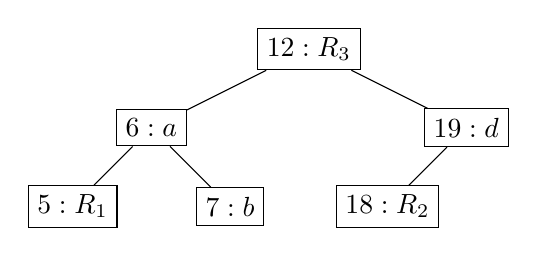
\begin{tikzpicture}
		
		\node[draw] (12) at (0,0) {$12: R_3$};
		\node[draw] (6) at (-2, -1) {$6: a$};
		\node[draw] (19) at (2, -1) {$19: d$};
		\node[draw] (18) at (1, -2) {$18: R_2$}; 
		\node[draw] (5) at (-3, -2) {$5: R_1$};
		\node[draw] (7) at (-1, -2) {$7: b$};
		
		\draw[-] (12) -- (6);
		\draw[-] (6) -- (5);
		\draw[-] (6) -- (7);
		\draw[-] (12) -- (19);
		\draw[-] (19) -- (18);
		
	\end{tikzpicture}
\end{figure}

Sei also ein Baum mit $n$ Elementen gegeben, so wie ein Intervall $[i..j]$, $i <= j$. Liegen nun $k$ Elemente, im Intervall $[i..j]$, so können alle diese Elemente insgesamt in $\mathcal{O}(k \log n)$ Laufzeit entfernt werden, da immer $\mathcal{O}(\log n)$ Laufzeit benötigt wird, um ein Element zu finden.

\subsection{Probleme}


Die Laufzeit ist durch die beschränkte Wahl der LCP-Intervalle, \texttt{RuleIntervalIndex} und die Verbesserte Regel-Datenstruktur, erheblich verbessert, aber es gibt trotzdem noch Probleme mit V3.

\subsubsection{Speicherverbrauch}
Da V3 als erste Version auch auf Datenmengen größer als 1MB tolerable Laufzeiten erzielt, stellt sich als nächstes das Problem des Speicherverbrauchs. Allein auf einer Datenmenge von 50MB, benötigte V3 schon etwa 6-8GB oder mehr.

\subsubsection{Effizienz von RuleInvervalIndex}

Außerdem ist \texttt{RuleIntervalIndex} nicht optimal. Viele der Operationen benötigen noch mehrere Anfragen an die darunterligende Predecessor-Datenstruktur.\\
Um etwa für einen Index $i$ den Intervall-Teil des Ersetzungsintervalls zu erhalten in dem $\texttt{i}$ liegt, muss zuerst ein $\texttt{predecessor(i)}$ Aufruf durchgeführt werden, um den Intervall-Teil $\texttt{part}$zu erhalten in dem $\texttt{i}$ liegt. Dann muss eine $\texttt{get(part.totalStart)}$ Anfrage durchgeführt werden, um den ersten Intervall-Teil zu erhalten.\\
Diese Anfrage kommt oft vor, da sie benötigt wird, um zu entscheiden, ob ein Vorkommen eines Musters ersetzt werden darf.

Dazu ist das markieren, also das einfügen neuer Ersetzungsintervalle noch kostspielig. Dies benötigt ebenfalls mehrere Anfragen an die Predecessor-Struktur. Außerdem müssen für das neu einzufügende Intervall $[start, end]$ alle Intervalle mit Startpositionen im Bereich $[start, end]$ durchlaufen werden, um diese potentiell zu ersetzen, falls diese weniger tief verschachtelt sind, als das neu einzufügende Intervall. Dies kann im Worst-Case lineare Laufzeit in der Länge der Eingabe bedeuten.

\subsubsection{Zu strenge Entscheidung ob Vorkommen ersetzt werden dürfen}

Ein weiteres Problem istbei der Entwicklung dieser Datenstrukturen aufgefallen. Es gibt fälle, in denen die bisher geschriebenen Algorithmen eine Ersetzung verbieten, obwohl diese eigentlich legal wäre.

Sei $p$ ein Muster mit Länge $k := |p|$. Bisher wird entschieden, ob eine Substitution von $p$ bei Index $i$ legal ist, indem geprüft wird, ob $\texttt{intervalContaining(i)}$ und $\texttt{intervalContaining(i + k - 1)}$ dieselben $\texttt{ruleId}$ und $\texttt{totalStart}$ besitzen, also die Start- und Endposition des neu entstehenden Ersetzungsintervalls in demselben Ersetzungsintervall liegen. Falls dies der Fall ist, ist eine Ersetzungs auch tatsächlich immer legal. Allerdings übersieht diese Berechung einen Fall:

Betrachten wir beispielsweise die folgende Grammatik für den String $abcdeabcd$:
\begin{align*}
	R_0 &\rightarrow R_1 c d e R_1 c d\\
	R_1 &\rightarrow a b\\
\end{align*}
Angenommen, als nächstes soll das Muster $abcd$ ersetzt werden (beachte, die Muster sind immer bezüglich des Eingabestrings, da das Suffix- und LCP array für diesen berechnet sind).
\texttt{RuleIntervalIndex} sieht hier folgendermaßen aus:
\begin{figure}[H]
	\centering
	\begin{tabular}{|c|c|c|c|} \hline
		$R_1$-$[0..1]$ & $R_0$-$[2..4]$ & $R_1$-$[5..6]$ & $R_0$-$[7..8]$ \\\hline
	\end{tabular}
\end{figure}

Das Muster $abcd$ kommt bei den Indizes $[0, 5]$ vor. Beide Ersetzungen sind offensichtlich legal, indem eine neue Regel $R_2 \rightarrow R_1cd$ eingeführt wird.\\ Versucht man aber nun mit der bisherigen Methode zu prüfen, ob die Ersetzung legal ist, so, erhält man:
\begin{align*}
	I_1 &:= \texttt{intervalContaining(0)} = R_1\text{-}[0..1]\\
	I_2 &:= \texttt{intervalContaining(0 + 4 - 1)} = R_0\text{-}[2..4]
\end{align*} 
Dabei ist dann $1 = I_1.ruleId \neq I_2.ruleId = 0$ und $0 = I_1.totalStart \neq I_2.totalStart = 2$. Die Ersetzung wird also verweigert, obwohl diese eigentlich legal wäre.\\
Diese Fälle treten ein, wenn das erste oder letzte Zeichen des zu ersetzenden Musters ein Nichtterminal ist (das Muster $abcd$ lag in der Grammatik bereits als das ersetzte $R_1 cd$ vor).

\texttt{RuleIntervalIndex} bietet zu diesem Zeitpunkt nicht die Daten um diesen Fall effizient korrekt zu entscheiden.

\section{AreaComp V4}

Dies ist nun die finale Version dieses Algorithmus und wird im größten Detail beschrieben.